\chapter{Metóda detekcie prebalených aplikácií Apk Analyzer}
\label{chap:metoda-detekcie-apk-analyzer}
V~rámci práce je navrhnutá metóda detekcie prebalených APK súborov. Navrhnutá metóda stavia na poznatkoch existujúcich výzkumov, a je založená predovšetkým na podobnosti zdrojových súborov obsiahnutých v~aplikáciách. Základom pre novonavrhnutú metódu sú práce \zv{FSquaDRA} a \zv{ImageStruct}. Primárnym cieľom novej metódy je vytvoriť spôsob detekcie prebalených aplikácií, ktorý je pomocou mobilnej aplikácie prístupný pre použitie širokej škále užívateľov systému Android.

\section{Motivácia a ciele}

Medzi existujúcimi riešeniami bolo identifikovaných niekoľko možných vylepšení, ktoré návrh novej metódy zohľadňuje. Tieto vylepšenia súvisia predovšetkým so sprístupnením tejto metódy používateľom.  Navrhnutá metóda sa zameriava na vylepšenie nasledujúcich oblastí:
\begin{itemize}
	\item Určenie, ktorá aplikácia je originál a ktorá prebalená kópia,
	\item Detekcia prebalených aplikácií pochádzajúcich výhradne z~alternatívnych obchodov,
	\item Kolaborácia užívateľov za účelom spresnenia detekčnej metódy,
	\item Dynamická aktualizácia dát potrebných na detekciu prebalených súborov.
\end{itemize}

\subsection*{Sprístupnenie užívateľom}

Známe metódy detekcie prebalených APK súborov (vrátane metód predstavených v~kapitole \ref{chap:zname-metody}) vykonávajú tzv. offline analýzu dát. Tieto metódy pracujú nad existujúcou databázou súborov, nad ktorou vykonávajú operácie s~cieľom identifikácie prebalených dvojíc. Offline metódy slúžia predovšetkým na vedecké účely, no môžu byť použité priamo obchodmi s~aplikáciami. V~súčasnosti však mnohé obchody vrátane \zv{Google Play} nie sú efektívne zabezpečené proti prebaleným aplikáciám~\cite{Zhauniarovich2013}. Užívatelia sú nútení chrániť svoje Android zariadenia pomocou antivírových programov. Napriek tomu, že niektoré antivírové a zabezpečovacie aplikácie môžu detekovať hrozby v~podobe prebalených aplikácií, v~súčasnosti (podľa vedomia autora) nie je rozšírená žiadna metóda zameriavajúca sa priamo na detekciu prebalených APK súborov na Android zariadení.

Metóda navrhnutá v~rámci projektu \zv{Apk Analyzer} predstavuje pre užívateľov ďalšiu možnosť ako ochrániť svoje zariadenie pred škodlivými aplikáciami. Cieľom je sprostredkovať užívateľom mechanizmus detekcie prebalených aplikácií priamo z~ich zariadenia. Tento spôsobo detekcie nebezpečných aplikácií môže byť použitý ako doplnok k~existujúcim nástrojom.


\subsection*{Určenie originálnej aplikácie a využitie pri alternatívnych zdrojoch}

Existujúce metódy detekcie prebalených aplikácií sú primárne zamerané na určenie vzťahu medzi dvomi aplikáciami. Takéto metódy dokážu detekovať nadmernú podobnosť dvojice aplikácií a rozhodnúť, či pochádzajú od rôznych autorov. Nástroje častokrát nedokážu určiť, ktorá z~týchto aplikácií je originál, a ktorá prebalená kópia. Väčšina nástrojov využíva predpoklad, že aplikácia pochádzajúca z~oficiálneho zdroja \zv{Google Play Store} je pravá a aplikácie z~alternatívnych zdrojov sú prebalené. Tento predpoklad však vo všeobecnosti platiť nemusí. Niektoré aplikácie sú distribuované výhradne pomocou alternatívnych kanálov. Existujúce metódy neumožňujú rozlíšenie medzi originálom a kópiou, v~prípade, že obe porovnávané aplikácie pochádzajú z~alternatívnych zdrojov. Keďže našim základným cieľom je ponúknuť detekciu prebalených aplikácií koncovému užívateľovi, je výsledok detekcie bez rozhodnutia ktorá aplikácia je originál a ktorá prebalená kópia nedostačujúci. 


Cieľom je poskytnúť užívateľovi odpoveď, ktorá ho informuje či je jeho aplikácia podľa systému \zv{Apk Analyzer} prebalená. 
Zámerom metódy \zv{Apk Analyzer} je využiť heuristiku počtu výskytov jednotlivých verzií aplikácií s~prirodzeným predpokladom, že na Android zariadeniach sa nachádza väčší počet originálnych aplikácií, ako ich prebalených kópií. 

\subsection*{Dynamickosť a kolaborácia}
Predstavené offline metódy pracujú nad statickou kolekciou aplikácií. Metódy využívané priamo v~obchodoch s~aplikáciami pracujú nad kolekciou aplikácií v~danom obchode. Za účelom vytvorenia metódy vychádzajúcej z~\zv{FSquaDRA} a \zv{ImageStruct} je nutné vytvoriť databázu aplikácií. Táto databáza však musí reflektovať zmeny v~aktuálne dostupných aplikáciách, pretože nové verzie a nové aplikácie sú vydávané dennodenne. 


Cieľom systému \zv{Apk Analyzer} je vytvorenie dynamickej databázy dát o~aplikáciách, na základe ktorej môže byť uskutočnená detekcia prebalených súborov.
Za týmto účelom je zámerom systému \zv{Apk Analyzer} zapojiť do tvorby databázy existujúcich aplikácií koncových užívatelov. Mobilná aplikácia, ktorá sprostredkováva detekciu prebalených aplikácií odošle dáta o~aplikáciách nainštalovaných na danom zariadení do centrálnej databázy systému \zv{Apk Analyzer}. Tento kolaboratívny spôsob zaručí neustálu aktualizáciu databázy. Čím viacej užívateľov je zapojených, tým väčšiu databázu sa podarí vytvoriť.

\section{Návrh metódy}
Návrh kompletného systému \zv{Apk Analyzer}, ktorý pozostáva z~mobilného klienta a serverovej časti obsahuje kapitola \ref{chap:apk-analyzer} . Táto kapitola sa zameriava predovšetkým na samotnú detekčnú metódu a tvorbu databázy, ktoré sa odohrávajú na strane serveru.

\subsection{Základný princíp detekcie prebalených aplikácií}
Mobilná aplikácia \zv{Apk Analyzer} odosiela dáta o~aplikáciách nainštalovaných na jednotlivých Android zariadeniach na server, ktorý ich ukladá do databázy. Pri detekcii sa použijú dáta uložené v~databáze. K~analyzovanej aplikácii sa vyhľadajú podobné aplikácie. Podobnosť je určená ako pomer obrázkov, ktoré dve aplikácie zdieľajú. Z~kolekcie aplikácií, ktoré zdieľajú veľkú časť obrázkov, a teda sú považované za rôzne verzie tej istej aplikácie je vybraný najčastejšie sa opakujúci digitálny podpis, ako identifikátor originálnej verzie. Ak je analyzovaná aplikácia podpísaná týmto kľúčom, je označená za dôveryhodnú. V~opačnom prípade systém upozorní užívateľa na prebalenú aplikáciu. 

\begin{figure}[htb]
  \begin{center}
    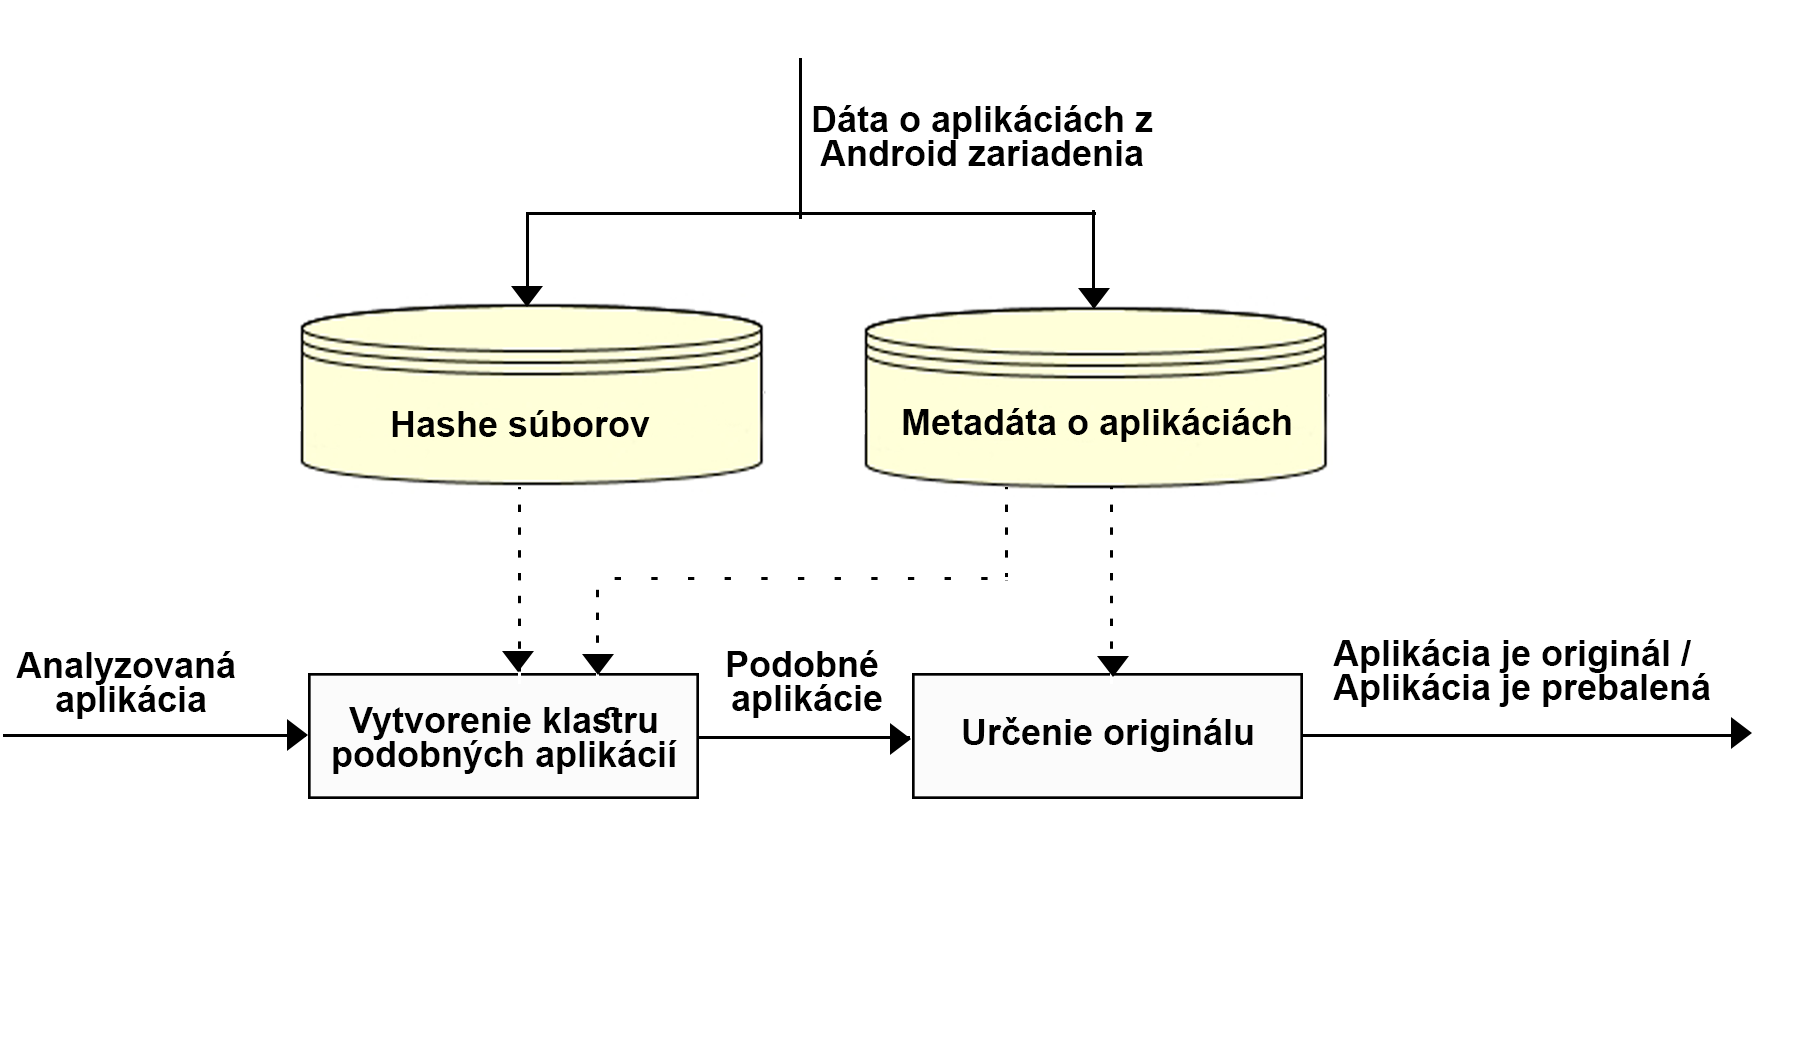
\includegraphics[width=130mm]{images/detection-overview.png}
  \end{center}
  \caption{Postup metódy Apk Analyzer}
  \label{fig:metódaApkAnalyzer}
\end{figure}

\subsection{Databáza aplikácií}

Základom detekcie prebalených aplikácií je databáza metainformácií o~aplikáciách. Dáta o~aplikáciách pochádzajú z~analýzy, ktorá je vykonaná na Android zariadeniach. Detailné informácie týkajúce sa analýzy aplikácií pomocou mobilnej aplikácie \zv{Apk Analyzer} sa nachádzajú v~kapitole \ref{chap:mobilna-aplikacia}. Mobilná aplikácia odosiela metadáta o~každej nesystémovej aplikácii na server.

 
\noindent Tento prístup poskytuje nasledujúce výhody:
\begin{itemize}
	\item \bod{Rozloženie výpočtovej záťaže} -- výpočtová záťaž spojená s~analýzou a reverzným inžinierstvom APK súborov je distribuovaná medzi mnohé Android zariadenia. Každé zariadenie analyzuje svoje nainštalované aplikácie. Hromadná centralizovaná analýza veľkého množstva aplikácií je výpočtovo a časovo náročná činnosť. Server nevykonáva dekompiláciu aplikácie, ale len ukladá dáta, ktoré mu odošle Android zariadenie.
	\item \bod{Dynamický vývoj databázy} -- klientska aplikácia odosiela na server všetky nesystémové aplikácie, vrátane aktualizovaných verzií. To zabezpečuje, že databáza aplikácií sa dynamicky vyvíja a obsahuje aj najnovšie aplikácie. Z~dôvodu udržovania aktuálnosti databázy nie je potrebný žiadny zásah administrátora.
\end{itemize}

\noindent Odosielané dáta o~nainštalovaných aplikáciách sú podmnožinou dát získaných analýzou APK súboru. Tieto dáta obsahujú základné metadáta ako napríklad meno balíka aplikácie, veľkosť APK súboru, hash certifikátu alebo počty jednotlivých komponent aplikácie. Okrem toho sú odosielané aj hashe a názvy všetkých rastrových obrázkových súborov obsiahnutých v~APK balíčku a taktiež bezpečnostné povolenia využívané aplikáciou. Kompletný zoznam všetkých uchovávaných atribútov aplikácie obsahuje príloha \ref{zbieraneDataPriloha}.

\subsubsection{\textbf{Identifikátor aplikácie}} 

Z~dôvodu efektivity vyhľadávania v~databáze je pre každú aplikáciu určený jej unikátny identifikátor. V~prípade, že majú dve aplikácie tento identifikátor rovnaký, ide o~úplne rovnakú aplikáciu a v~databáze ju server ukladá len raz.


\noindent Na tvorbu tohto identifikátoru sú použité nasledovné atribúty APK balíčka: 
\begin{itemize}
	\item \bod{meno balíka aplikácie} -- z~pohľadu systému Android identifikuje aplikáciu. Pokiaľ majú dve aplikácie rovnaké meno balíka, jedná sa o~rôzne verzie tej istej aplikácie,
	\item \bod{hash certifikátu aplikácie} -- unikátne identifikuje autora aplikácie,
	\item \bod{hash súboru Classes.dex} -- reprezentácia zdrojového kódu aplikácie,
	\item \bod{hash súboru Resources.arsc} -- reprezentácia skompilovaných zdrojových súborov aplikácie,
	\item \bod{hash súboru AndroidManifest.xml} -- reprezentácia hlavného metasúboru,
	\item \bod{kombinovaný hash všetkých obrázkov} -- identifikuje kolekciu obrázkov aplikácie,
	\item \bod{počet obrázkových súborov},
	\item \bod{počet xml súborov}.
\end{itemize}
V~prípade, že majú dve aplikácie rovnaký identifikátor, je zaručené, že pochádzajú od jedného vydavateľa, ich zdrojový kód, skompilované zdrojové súbory, metadáta a všetky  obrázky sú identické. 

\subsubsection{\textbf{Počet výskytov aplikácie}}
Dôležitým aspektom pri detekcii prebalených aplikácií je počet výskytov jednotlivých verzií aplikácií. Túto metriku systém využíva pri určení, ktoré aplikácie sú originály a ktoré prebalené imitácie. Preto je dôležité identifikovať, z~akého zariadenia dáta o~aplikácii pochádzajú. Za týmto účelom je použitý unikátny identifikátor zariadenia \zv{AndroidID}. Server si ku každej aplikácii pamätá všetky zariadenia, z~ktorých bola daná aplikácia nahraná, a taktiež uchováva informácie z~akého zdroje bola aplikácia na dané zariadenie nainštalovaná.


\subsubsection{\textbf{Eliminácia obrázkov z~často používaných knižníc}}
\label{sec:eliminacia-kniznic}
Algoritmus detekcie prebalených aplikácií zisťuje počet rovnakých obrázkových súborov v~rozdielnych aplikáciách. Aplikácie štandardne obsahujú viacero obrázkov, ktoré pochádzajú z~často používaných knižníc. Medzi často používané knižnice patria predovšetkým knižnice zaručujúce spätnú kompatibilitu medzi verziami systému Android, známe ako \zv{Google support libraries}. Obrázkové súbory pochádzajúce z~knižníc nemôžu byť použité algoritmom pre detekciu podobnosti. Takéto obrázky necharakterizujú konkrétne aplikácie. Z~tohto dôvodu je potrebná ich eliminácia, ktorá sa odohráva pri ukladaní aplikačných metadát do databázy. Každá z~knižníc je dostupná vo viacerých vydaniach. Obrázky sú medzi týmito vydaniami upravované, avšak ich názvy zostávajú nezmenené. Filtrovanie obrázkov na základe ich presných hashov zadaných administrátorom by si vyžadovalo pravidelnú aktualizáciu a z~dlhodobého hľadiska by bolo ťažko udržateľné. Z~tohto dôvodu náš algoritmus na základe mien súborov dynamicky buduje zoznam hashov obrázkov z~knižníc. Pri vkladaní záznamu o~jednom obrázkovom súbore sa najskôr skontroluje názov súboru. V~prípade, že zodpovedá názvu súboru z~často používaných knižníc, databáza hashov súborov z~knižníc sa rozšíri o~spracovávaný obrázok a tento obrázkový súbor nie je uložený medzi obrázky danej aplikácie. V~opačnom prípade sa aplikácia pokúsi vyhľadať hash súboru v~databáze hashov obrázkov z~knižníc. V~závislosti na výsledku tejto operácie je následne súbor ignorovaný alebo pridaný medzi obrázky danej aplikácie.

\subsubsection{\textbf{Dátový model}}
Návrh dátového modelu zodpovedá štruktúre ukladaných dát. Vzhľadom k~požiadavkám kladeným na systém Apk Analyzer je použité riešenie prezentované na ERD diagrame \ref{fig:detectionDbErd}. 

\begin{figure}[htb]
  \begin{center}
    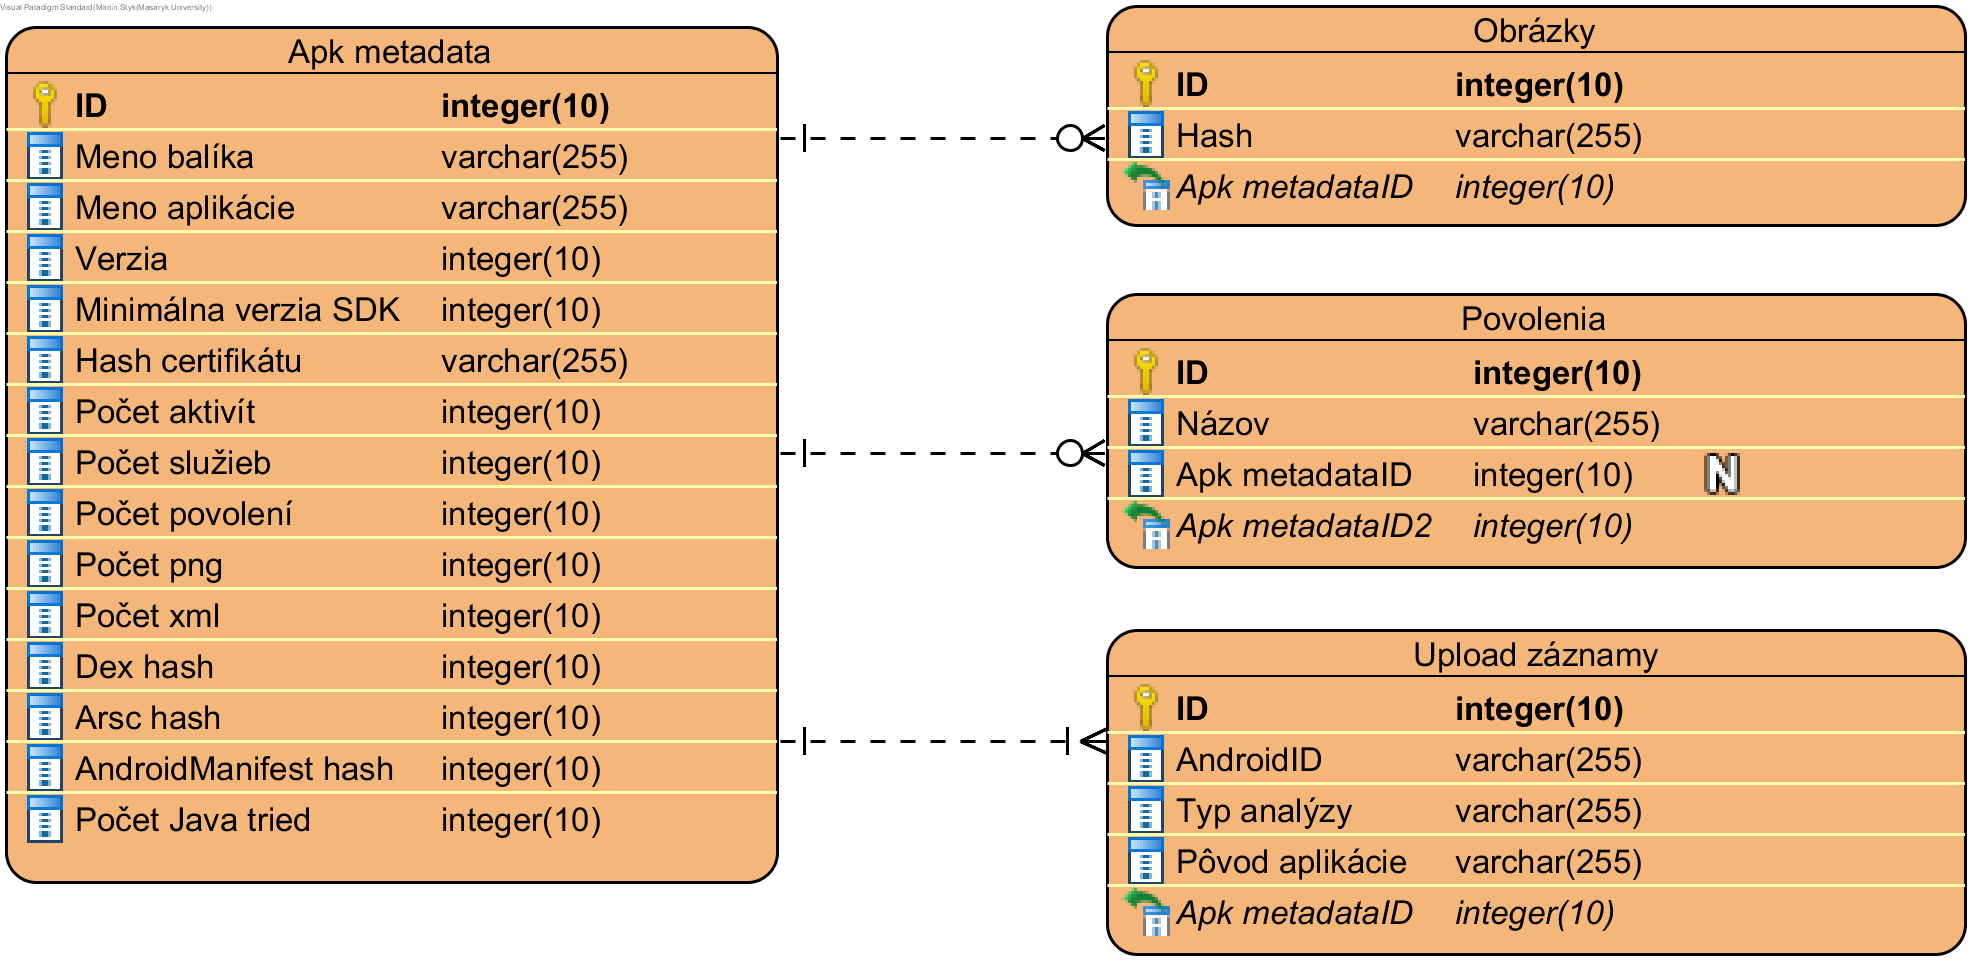
\includegraphics[width=130mm]{images/detection-db-erd.png}
  \end{center}
  \caption{Dátový model ukladajúci informácie o~aplikáciách}
  \label{fig:detectionDbErd}
\end{figure}

Pri tvorbe dátového modelu je potrebné zohľadniť požadovanú výkonnosť aplikácie. Za účelom optimalizácie výkonnosti nemá dátový model normalizovanú dátovú schému. Niektoré atribúty v~tabuľke \zv{Apk metadata} sú duplicitné, a môžu byť získané pomocou dotazov na iné tabulky. Z~dôvodu optimalizácie výkonnosti sú však tieto dáta uložené priamo v~tabulke \zv{Apk metadata}.
Ďalším porušením normalizácie je vzťah medzi tabuľkou \zv{Apk metadata} a \zv{Obrázky}, respektíve \zv{Apk metadata} a \zv{Povolenia}. V~systéme môže nastať situácia, že jeden súbor, prípadne jedno povolenie je zdieľané medzi viacerými aplikáciami. V~tom prípade by mal byť medzi týmito entitnými množinami použitý vzťah $N : N$. Takýto prístup by vyžadoval použitie spojovacej tabuľky, čo by malo negatívny vplyv na výkonnosť. Nad databázou vykonáva systém \zv{Apk Analyzer} iba operácie dotazovania a vkladania nových záznamov. Negatívne dôsledky nenormalizovanej databázovej schémy by spôsobili problémy predovšetkým pri operáciách \zv{update} a \zv{delete}. Medzi negatíva zvoleného prístupu patrí zvýšená veľkosť ukladaných dát. Tieto nedostatky sú však vyvážené vyššou výkonnosťou. Vloženie jedného záznamu o~APK súbore do existujúcej databázy trvá približne $100\, ms$. Pri použití normalizovanej schémy zaberie táto operácia dvadsaťnásobne viac času.  

\subsection{Detekcia prebalených aplikácií}

Základným obmedzením kladeným na metódu detekcie prebalených APK súborov je využitie dát, ktoré sú získané analýzou vykonávanou klientskou aplikáciou priamo na Android zariadení. S~tým je spojených viacero limitácií. 
Metódy využívajúce analýzu zdrojového kódu aplikácií sú výpočtovo náročné. Extrakcia dát zo súboru \zv{classes.dex} a vytvorenie identifikátora aplikácie na základe týchto dát predstavuje netriviálnu výpočtovú záťaž~\cite{Zhou2012b}. Viaceré výzkumy ukázali, že metódy detekcie prebalených aplikácií založené na podobnosti súborov vytvárajúcich vzhľad aplikácie dosahujú provnateľné výsledky ako metódy využívajúce analýzu zdrojového kódu~\cite{Gadyatskaya2016,Zhauniarovich2014, ImageStruct}.

Na rozdiel od metódy \zv{ImageStruct} naša metóda neextrahuje z~obrázkových súborov dáta, ale využíva hash celého súboru. Porovnávanie je teda založené na presnej binárnej zhode. Získanie charakteristických informácií obrázka podobne ako v~metóde \zv{ImageStruct} nie je možné, pretože klientska aplikácia nemá priamy prístup k~obrázkovým súborom iných aplikácií. Preto sa naša metóda spolieha na predpoklad, že pri prebaľovaní aplikácií sa obrázkové súbory často nemenia. 
V~porovnaní s~metódou \zv{FSquaDRA} nepoužíva \zv{Apk Analyzer} pri porovnaní všetky súbory, ale len rastrové obrázky.

Samotný algoritmus detekcie prebalených súborov dostane na vstup aplikáciu, o~ktorej má rozhodnúť, či je prebalená alebo nie. Algoritmus sa skladá z~viacerých krokov.

\subsubsection{\textbf{Detekcia klastru podobných aplikácií}} 

V~prvom kroku algoritmus nájde všetky aplikácie, ktoré spĺňajú definované kritériá zhody aplikácií. Tieto kritériá pozostávajú z~podobnosti metadát a zhody obrázkových súborov. 
Podobnosť metadát je použitá za účelom zefektívnenia vyhľadávania podobných aplikácií. Algoritmus sa rozhoduje na základe metadát, ktoré nemôžu byť pri prebaľovaní ľahko zmenené, respektíve z~výsledkov predchádzajúcich výskumov vyplýva, že ich útočníci často nemenia. \newline \noindent Algoritmus používa nasledujúce atribúty:
\begin{itemize}
	\item počet \zv{xml} súborov v~aplikácii
	\item počet obrázkových súborov v~aplikácii
	\item celkový počet súborov
	\item počet Java tried v~aplikácii
\end{itemize}

Všetky z~týchto atribútov sú číselné. Ako podobné aplikácie sú na základe týchto atribútov označené také aplikácie, ktorých hodnoty týchto atribútov sú v~rozmedzí $\pm 20$ \% od hodnôt analyzovanej aplikácie. Hodnota 20 \% bola určená na základe experimentov nad databázou APK súborov. Tieto pokusy ukázali ukázali, že zmena tohto parametru na vyššie hodnoty nemá zásadný vplyv na výsledky detekcie. Pri nastavení povoleného rozmedzia na 50 \% stúpol počet detekovaných aplikácií o~3\%.

Aplikácie, ktorých metadáta sú vyhodnotené ako podobné, sú následne porovnané s~aplikáciou ktorej detekcia prebieha. Toto porovnanie je založené na zhode obrázkových súborov v~týchto APK balíčkoch. Algoritmus neberie do úvahy obrázky pochádzajúce z~knižníc, pretože takéto obrázky necharakterizujú jednotlivé aplikácie.  Koeficient podobnosti je určený pomocou \zv{Jaccardovej metódy}.

\[ similarity(app_1, app_2) = \frac{|app_{1}images \cap app_{2}images|} { app_{1}images} \]

Hodnota Jaccardovho koeficientu, nad ktorou sú aplikácie považované za zhodné je odvodená z~metódy \zv{FSquaDRA} a naväzujúcich prác. Algoritmus APK balíčky ako rôzne verzie jednej aplikácie, ak je Jaccardov index podobnosti vyšší ako $0,7$.

Výstupom prvej časti algoritmu je skupina aplikácií, ktoré algoritmus klasifikuje ako nadmieru podobné. Takéto aplikácie považujeme za rôzne druhy jednej aplikácie.

\begin{figure}[htb]
  \begin{center}
    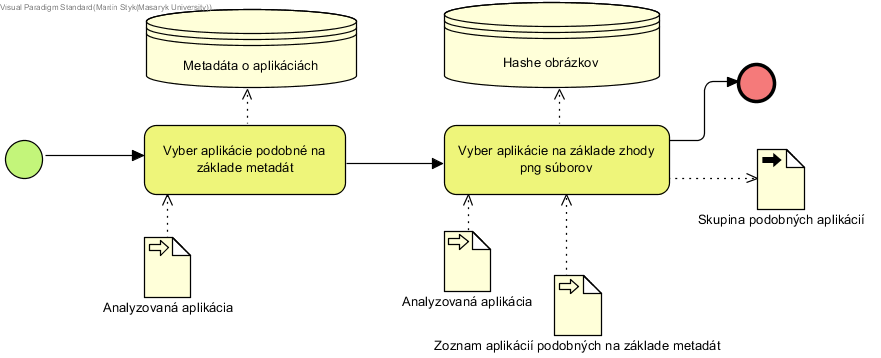
\includegraphics[width=130mm]{images/detection-cluster.png}
  \end{center}
  \caption{Postrup tvorby klastru podobných aplikácií}
  \label{fig:detectionClustering}
\end{figure}
\subsubsection{\textbf{Identifikácia originálu}} 
V~predchádzajúcom kroku identifikuje algoritmus nadmieru podobné aplikácie. Aplikácia, ktorej detekcia prebieha je s~aplikáciami z~tejto skupiny zvyčajne v~jednom z~nasledujúcich vzťahov:
\begin{itemize}
	\item rôzne verzie jednej aplikácie
	\item upravené / prebalené aplikácie
	\item iné (false positive)
\end{itemize}
V~takejto skupine sa môžu vyskytovať aj aplikácie, ktoré nie sú inou verziou alebo kópiou aplikácie, ktorej detekcia prebieha. Popis možných chýb a nedostatkou tejto metódy obsahuje sekcia \ref{sec:hodnotenie}.

Na základe digitálneho podpisu APK balíčka vieme rozhodnúť, do ktorej z~týchto kategórií aplikácia patrí. V~prípade zhody certifikátu, ktorým sú aplikácie podpísané, ide o~dve rôzne verzie jednej aplikácie, ktoré pochádzajú od jedného vydavateľa. V~prípade podpisu rôznymi certifikátmi považujeme jednu z~týchto aplikácií za prebalenú, pretože aplikácie pochádzajú od rôznych vydavateľov a na základe ich nadmiernej podobnosti sú považované za jednu logickú aplikáciu.

Metóda detekcie prebalených aplikácií implementovaná v~rámci systému \zv{Apk Analyzer} využíva heuristiku založenú na početnosti výskytu aplikácií. Základom tejto metódy je pozorovanie, že na Android zariadeniach je nainštalovaných viac originálnych aplikácií, ako ich prebalených kópií.

Aplikácie sú rozdelené do skupín podľa ich digitálneho podpisu. Aplikácia, ktorej detekcia prebieha, je označená ako originálna v~prípade, že je podpísaná kľúčom, ktorým je podpísaná väčšina APK súborov v~klastri podobných aplikácií.  V~opačnom prípade vyhodnotí algoritmus túto aplikáciu ako prebalenú kópiu. Pri určovaní počtu aplikácií sa zohľadňuje počet výskytu jednotlivých verzií na rôznych zariadeniach. 

V~prípade, že kolekcia podobných aplikácií neobsahuje záznamy minimálne o~piatich aplikáciách prítomných na rôznych zariadeniach, proces je ukončený s~odpoveďou oznamujúcou nedostatok dát pre vykonanie spoľahlivej detekcie pôvodu aplikácie.

\begin{figure}[htb]
  \begin{center}
    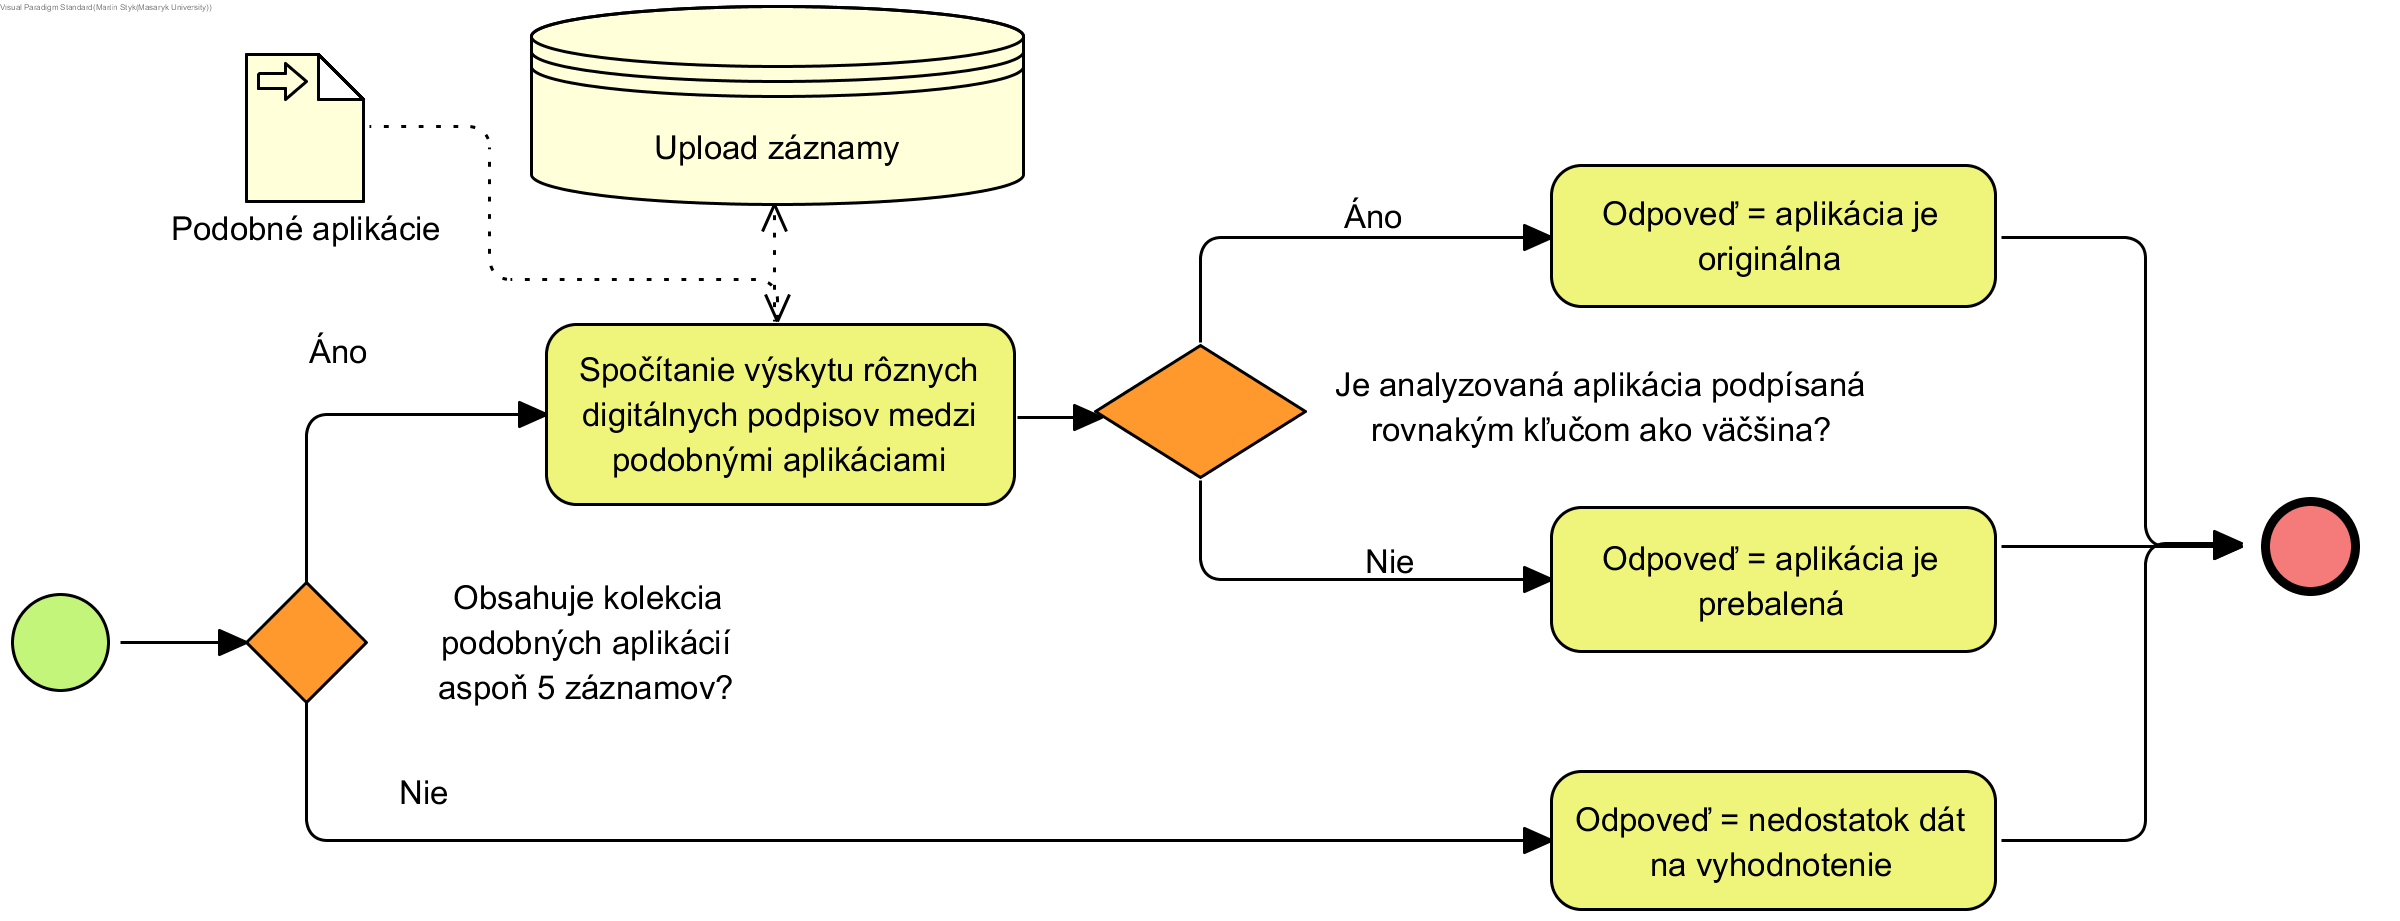
\includegraphics[width=130mm]{images/detection-original.png}
  \end{center}
  \caption{Postup určenia výsledku detekcie}
  \label{fig:detectionOriginal}
\end{figure}

\section{Predpoklady navrhnutej metódy}
Navrhnutá metóda využíva pri detekcii prebalených aplikácií viacero dôležitých predpokladov.

\subsection*{V obehu je viac originálnych aplikácií ako prebalených}
Tento predpoklad vychádza zo základného princípu prebalených aplikácií, ktoré využívajú popularitu originálnej aplikácie za účelom šírenia škodlivej funkcionality.

\subsection*{Obrázkové súbory je možné použiť na detekciu prebalených aplikácií}
Metóda detekcie prebalených APK súborov \zv{ImageStruct} založená na porovnaní vlastností obrázkov ukázala, že výskyt rovnakých obrázkov je silným indikátorom prebalenia aplikácie. Funkčnosť a presnosť tohto prístupu bola overená prostredníctvom porovnania s~metódou založenou na analýze zdrojového kódu \cite{ImageStruct}. Podobné zistenia sú prezentované aj v~rámci práce \zv{FSquaDRA}, ktorá detekuje prebalené kópie na základe porovnania všetkých súborov aplikácií~\cite{Zhauniarovich2014}. V~rámci rozširujúcej evaluácie metódy \zv{FSquaDRA} bolo zistené, že presnosť detekcie je možné zvýšiť pomocou vzájomného porovnanie súborov rovnakého typu~\cite{Gadyatskaya2016}. Tento prístup sme použili aj v~metóde \zv{Apk Analyzer}. Viacero známych metód sa pri identifikácií typov súborov spolieha na štandardnú štruktúra APK balíčka. Práca vyhodnocujúca metódu \zv{FSquaDRA} využíva predpoklad, že obrázkové súbory sa nachádzajú v~štandardnom priečinku \cesta{res/drawable}. Súborová štruktúra APK balíčka môže byť predmetom obfuskácie, ktorú využívajú vývojári za účelom skomplikovania reverzného inžinierstva, a útočníci prebaľujúci aplikácie za účelom odlíšenia kópie od originálu. Z~tohto dôvodu používa náš prístup podobnosť všetkých súborov vo formátoch \zv{png}, \zv{bmp}, \zv{webp}, \zv{jpg} a \zv{gif}. Intuícia za týmto návrhom je založená na pozorovaní, že pri obfuskácii môžu byť zmenené názvy priečinkov a súborov, avšak typ súboru zostáva rovnaký. Tabuľka \ref{images-apk} ukazuje zastúpenie formátov obrázkových súborov v~analyzovanej vzorke 16\,700 aplikácií.
\begin{table}[]
\centering
\label{images-apk}
\begin{tabular}{|l|c|c|}
\hline
\textbf{Formát} & \textbf{Priemerný počet}  & \textbf{Medián}         \\ \hline
png             & 369                       & 144         \\
jpg             & 7                         & 0                 \\
gif             & 0,4                       & 0             \\
webp            & 0,4                       & 0         \\
bmp             & 0,1                       & 0         \\
\hline
\end{tabular}
\caption{Obrázkové súbory v~APK balíčku}
\end{table}

\subsection*{Pri prebaľovaní aplikácií sú obrázkové súbory nepozmenené}
Navrhnutá metóda detekcie porovnáva obrázky na základe ich hashov. Aj malá úprava obrázku spôsobí kompletnú zmenu jeho hashu. Preto je pre navrhnutú metódu detekcie kľúčové, aby obrázky v~prebalenej aplikácií zostali nezmenené. Skúmaním zmien vykonávaných pri prebaľovaní aplikácie sa zaoberala Olga Gadyatskaya a kolektív v~roku 2016~\cite{Gadyatskaya2016}. V~tomto období boli už k~dispozícií viaceré metódy využívajúce na detekciu prebalených aplikácií podobnosť zdrojových súborov, vrátane metód \zv{FSquaDRA} a \zv{ImageStruct}. Napriek tomu výsledky výzkumu ukázali, že pri prebaľovaní zostávajú zdrojové súbory zvyčajne nemodifikované a útočníci najčastejšie modifikujú súbor \zv{classes.dex} a \zv{AndroidManifest.xml}. Tento fakt môžeme vysvetliť tak, že metódy založené na podobnosti zdrojových súborov nie sú v~praxi veľmi rozšírené a útočníci ich nepovažujú za hrozbu ani napriek ich preukázanej kvalite. Preto sa pri prebaľovaní sústredia najmä na zmeny v~zdrojovom kóde, a ostatné súbory zostávajú nepozmenené. Nasledujúca tabuľka \ref{repacakged-changes} zobrazuje typy súborov a pravdepodobnosť, že súbor daného typu je modifikovaný v~prebalenej aplikácii. Tento prístup však predstavuje limitáciu z~pohľadu budúcnosti. V~prípade, že útočníci začnú aplikovať zmeny v~obrázkových súboroch, môžu efektívne zabrániť detekcií pomocou narhnutého algoritmu. V~súčasnosti nie sú obrázkové súbory pri prebaľovaní často modifikované a teda ich priame binárne porovnanie môže byť použité za účelom nájdenia prebalených aplikácií.

\begin{table}[]
\centering
\label{repacakged-changes}
\begin{tabular}{|l|l|}
\hline
\textbf{Pravdepodobnosť modifikácie} & \textbf{Typ súboru}          \\ \hline
0,0212                                      & audio video         \\
0,0624                                      & raw                 \\
0,0731                                      & obrázok             \\
\multicolumn{2}{|c|}{...} \\
0,8476                                      & Resources.arsc      \\
0,9066                                      & AndroidManifest.xml \\
0,9227                                      & zdrojový kód        \\
\hline
\end{tabular}
\caption{Zmeny v~prebalených APK súboroch}
\end{table}

\subsection*{Nastavenia detekcie na základe predchádzajúcich výskumov}
Známe výskumy prebalených APK súborov pracujú nad offline databázou aplikácií. Funkčnosť a presnosť týchto metód je vyhodnotená prostredníctvom porovnania výsledkov s~inými algoritmami. Na základe experimentov sú určené parametre detekcie, ktoré eliminujú nesprávne výsledky algoritmu. V~prípade našej metódy je situácia komplikovanejšia, pretože našu databázu netvoria celé APK súbory, ale len niektoré metadáta. Nie je teda možné spustiť nad týmito dátami iné metódy detekcie, a nastaviť tak parametre algoritmu, ktoré ovplyvňujú výsledky detekcie. Z~metadát o~jednotlivých aplikáciách nie je možné rozhodnúť, či je daná aplikácia originál, alebo prebalená verzia.  Z~toho dôvodu sa navrhnutá metóda vo veľkej miere opiera o~už existujúce výskumy a preberá ich závery a odporúčané parametre detekcie. 

\section{Hodnotenie}
\label{sec:hodnotenie}
Implementovaná metóda bola nasadená v~produkčnom prostredí a je dostupná užívateľom. Táto sekcia hodnotí hlavné plusy a limitácie navrhnutej metódy detekcie prebalených aplikácií.

Implementovaná metóda v~praxi ukázala že dokáže identifikovať aplikácie, ktoré môžu byť potenciálne prebalené. Server zaznamenal celkovo TODO požiadavok na detekciu prebalených aplikácií. Z~tohto poču bolo TODO aplikácií vyhodnotených ako originálne verzie, TODO ako potenciálne prebalené a v~TODO prípadoch nemal server dostatok dát na určenie výsledku detekcie. GRAF TODO.

Zdieľaná databáza obsahuje informácie o~TODO aplikáciách. Požiadavka na detekciu prebalenej aplikácie je štandardne vyhodnotená do tridsiatich sekúnd. Aplikácií pre platformu Android existuje veľké množstvo. Samotný obchod \zv{Google Play} obsahuje v~súčasnosti viac ako 3,5 milióna aplikácií. V~prípade ďalšieho rozširovania metódy detekcie prebalených APK súborov \zv{Apk Analyzer} je potrebná výrazne robustnejšia a drahšia infraštruktúra. Aktuálne je riešenie implementované nad jednou inštanciou databázy \zv{Postgres}. Pri objeme dát, ktoré aplikácia aktuálne obsahuje je výkonnosť SQL databázového servera dostačujúca. V~prípade, že systém bude aj naďalej rásť, je možné využiť na ukladanie zoznamu hashov obrázkov systém \zv{Redis}, ktorý výrazne zvýši rýchlosť detekcie prebalených aplikácií. 

Jedným z~najzásadnejších prínosov tejto práce je sprostredkovanie detekcie prebalených aplikácií užívateľom. Implementovaná metóda využíva poznatky z~výzkumov z~oblasti prebalených aplikácií. Na základe týchto znalostí ponúka možnosť detekcie koncovým užívateľom a tým prepája vedecké štúdie s~praktickým využitím. 

Vďaka využitiu dynamickej databázy aplikácií, ktorú rozširujú samotný užívatelia, je detekčná metóda schopná vyhodnotiť aj najnovšie aplikácie.

\subsection{Limitácie}
Počas implementácie a nasadenia tejto metódy boli identifikované viaceré skutočnosti, ktoré môžu obmedziť využiteľnosť implementovanej metódy. Niektoré z~týchto obmedzení sa podarilo eliminovať.

\subsubsection{\textbf{Knižnice}}
V~prípade, že viaceré aplikácie používajú rovnaké knižnice, ktoré obsahujú obrázkové súbory, môžu tieto obrázky ovplyvniť výsledok detekcie. Implementovaná metóda sa s~obrázkami z~knižníc dokázala čiastočne vysporiadať pomocou odfiltrovania dát, ktoré zodpovedajú obrázkovým súborom pochádzajúcim z~často sa vyskytujúcich knižníc. Postup elimininácie takýchto súborov obsahuje sekcia \ref{sec:eliminacia-kniznic}. Na základe tohto algoritmu bolo eliminovaných 12\,500 TODO binárne rôznych obrázkov. Celkovo bolo eliminovaných 25 miliónov TODO obrázkových súborov. Ekosystém platformy Android však obsahuje veľké množstvo knižníc. Nové knižnice, prípadne nové vydania existujúcich knižníc sú publikované každodenne. Nie je preto možné vylúčiť, že v~prípade zhody jednej alebo viacerých knižníc, môže dojsť k~chybnej detekcií

\subsubsection{\textbf{Aplikácie bez výraznej vizuálnej identity}}
Väčšina často používaných aplikácií má svoju výraznú a nezameniteľnú vizuálnu identitu. Niektoré z~dostupných aplikácií však obsahujú veľmi malé množstvo multimediálnych súborov. V~prípade takýchto aplikácií je detekcia prebalenia na základe obrázkových súborov značne limitovaná.

\subsubsection{\textbf{Rôzne verzie APK súboru pre rôzne zariadenia}}
Prirodzeným predpokladom pri detekcií podobnosti aplikácií je, že viaceré verzie jednej aplikácie vyhodnotí algoritmus ako podobné. Tento predpoklad platí zvyčajne len pri jednoduchších aplikáciách. V~prípade komplexných aplikácií ako \zv{Facebook} alebo  aplikácie od spoločnosti \zv{Google} tento predpoklad platiť nemusí. \zv{Google Play} podporuje distribúciu viacerých verzií jednej aplikácie na základe typu a konfigurácie zariadení. V~praxi obsahuje vydanie jednej aplikácie na \zv{Google Play} viacero APK súborov. Pri inštalácii vyberie \zv{Google Play} APK balíček na základe parametrov daného zariadenia, najčastejšie podľa úrovni Android API a veľkosti obrazovky. Jednotlivé APK súbory sú optimalizované pre dané zariadenia. Z~tohto dôvodu sa jedna verzia aplikácie určenej pre tablet a aplikácie určenej pre mobilný telefón nemusí na základe obrázkov a metadát zhodovať. 
Táto skutočnosť však pre detekčnú metódu nepredstavuje výrazné riziko. Útočník musí vždy prebaliť niektoré z~distribuovaných APK súborov. Za predpokladu, že v~takto prebalenom súbore nemení existujúce obrázky je tento súbor detekovaný ako podobný s~originálnym APK súborom pre danú konfiguráciu zariadenia. Je však potrebné uvedomiť si, že nie všetky rôzne vydania aplikácie sú odhalené ako podobné aplikácie~\cite{MultipleApks}.

\subsubsection{\textbf{Zmeny obrázkových súborov}}
Metóda je postavená na základoch aktuálnych poznatkov, ktoré odhaľujú, že pri prebaľovaní aplikácií zvyčajne zostávajú zdrojové súbory nezmenené. V~prípade rozšírenia metód využívajúcich podobnosť zdrojových súborov je pravdepodobné, že útočníci začnú aplikovať výraznejšie zmeny v~rôznych súboroch obsiahnutých v~APK balíčku. Výrazná zmena počtu súborov v~balíčku alebo úpravy obsiahnutých obrázkov predstavujú spôsob, akým je možné navrhnutú metódu znefunkčniť. Avšak v~súčasnosti takéto zmeny vykonávané nie sú a navrhnutá metóda je schopná odhaliť prebalené aplikácie.
\\
\\
Popísané limitácie odhaľujú slabiny implementovanej metódy detekcie prebalených aplikácií. Napriek týmto nedostatkom však koncept identifikácie kópií originálnej aplikácie založený na podobnosti výzoru dokáže detekovať prebalené aplikácie. Tento prístup je vhodný ako doplnok k~existujúcim metódam vychádzajúcich z~podobnosti vzoriek inštrukcií aplikácie.


